\documentclass[twocolumn]{revtex4}
\usepackage{graphics,graphicx,epsfig,amsmath,multirow,gensymb,commath,textcomp,natbib,blindtext,mhchem,tabularx,array,makecell,threeparttable,amssymb,relsize,csquotes}
\usepackage{listings}
\usepackage[a4paper, left=1.85cm, right=1.85cm, top=1.85cm, bottom=1.85cm]{geometry}   
\usepackage[normalem]{ulem}
\newcommand{\squeezeup}{\vspace{-2.5mm}}

\usepackage{lipsum}

\def\bibsection{\section*{\refname}} 
\renewcommand{\thesubsection}{\alph{subsection}}

\renewcommand\theadalign{bc}
\renewcommand\theadfont{\bfseries}
\renewcommand\theadgape{\Gape[4pt]}
\renewcommand\cellgape{\Gape[4pt]}

\begin{document}

\textheight=26.385cm
%Change textheight as the last resort...

\title{Constraining the geometry of the Universe using Type Ia supernovae}
 
\author{Jacky Cao, Group C3, Physics Problem Solving \\ Date of report: 28/02/2018}

\begin{abstract}              
Type Ia supernovae have the unique trait of being standard candles, their light curves can be used in cosmology to calculate and constrain cosmological parameters. In observing Type Ia supernovae and fitting model light curves to such data one can attempt to derive such values. We have monitored, collected, and analysed data for supernova explosions over a period of 34 days. A $16''$ and a $0.5$ m telescope situated in Durham and La Palma was used for this project. After calculating the magnitudes for a Type Ia (2017hhz) and Type Ia-91bg (2017hle) supernova object, we fitted template light curves with the Python program, \textit{SNooPy}. The quality of fit for the program's \texttt{fit()} function was deemed to be acceptable in accordance to the average reduced $\chi^2$ values calculated for the B and V photometric bands, $\chi^2_{\nu,B} \approx 1.38$ and $\chi^2_{V,\nu} \approx 2.95$ - a good fit requiring $\chi^2_{\nu} \approx1$. The distance modulus to the supernova 2017hhz was calculated by SNooPy to be $36.121\pm0.106$ mag, using this value we were able to compute $H_0=70\pm20$ km s$^{-1}$ Mpc$^{-1}$. However, the quoted error negates the meaning of $H_0$ as it is too large of an uncertainty. In improving the accuracy and uncertainties we suggest that more observations of the supernovae were required, and constraining values should be used for the parameters in SNooPy's templates.
\end{abstract}

\maketitle

\vspace{-3ex}
\section{Introduction and Theory} 
\vspace{-2ex}
In cosmology, one can argue that one of the most important observable events are supernova explosions. As a massive main sequence star runs out of nuclear fuel to burn, the equilibrium configurations which initially provided structure will cease to exist. What follows is a cataclysmic supernova explosion \cite{longair}. 

We can generally class supernova explosions into two separate groups, Type I and Type II supernovae. The main distinction arises due to the fact that Type I's have an optical spectra which contains no Balmer hydrogen features, whilst Type II supernovae do contain this hydrogen feature \cite{mod_ast}. 

Within these two subclasses there are further divisions which can be characterised through their spectra and through features as found in their light curves \cite{obs_phys_class_sn}. Light curves are a way to show the evolution of a supernova's magnitude as time passes. With two of the subclasses of Type II supernovae, Type II-L and Type II-P, they have been classed by features of their respective light curves: a rapid linear decrease in magnitude and constant magnitude \cite{mod_ast}.

For the application of supernovae in cosmology, we must turn to supernovae of the Type Ia variety and to the light curves that they produce. 

\vspace{-3ex}
\subsection{Type Ia Supernovae}
\vspace{-2ex}
It is generally accepted that the light curves of Type Ia supernovae are homogeneous \cite{posn}, this means that they can be utilised as standard candles, therefore allowing us another measure of cosmic distance. 

Their homogeneity arises due to the mechanism behind their explosion. The progenitor system for Type Ia's consist of a binary system with a white dwarf and another star which has a mass close towards the Chandrasekhar limit of $1.4 M_{\odot}$ \cite{mod_ast, posn}. The white dwarf accretes matter from it's companion until it itself reaches this critical mass limit. After this point we would then expect the primary white dwarf to collapse into a neutron star, however this is not the case. Instead, we find that a supernova explosion occurs due to a disruption to it's internal structure.

It is currently understood that as the primary white dwarf star accretes matter it heats up and produces thermonuclear energy. This energy which is achieved in the stellar interior at a temperature of $10^9$ K disrupts the electron degeneracy pressure. The star becomes gravitationally unstable due to the disruption from the nuclear energy, a total collapse into a neutron star is thus prevented \cite{longair, posn}.

This particular mechanism can thus be used to attribute for the standard profile of Type Ia light curves. Using these graphs, the maximum B photometric band magnitude can be obtained from the following equation,
\begin{equation}
M_{\max}(B)=-21.726+2.698\Delta m_{15}(B),
\end{equation}

where $\Delta m_{15}(B)$ is the decline rate parameter or Phillips' parameter \cite{high_en_astro}. This is defined as the mean rate of decline of the B band light curve from peak light to 15 days after the maximum had been achieved \cite{abs_phil}. This parameter relates the apparent magnitude to time and provides a way to compare and contrast different Type Ia supernovae. 

With values for the absolute magnitude of Type Ia supernovae and with obtained values of redshift from spectroscopic observations of them, the distance to them can then be calculated using the following equation, 
\begin{equation}
\mu = 5 \log_{10}(d) - 5,
\end{equation}

where $\mu$ is the distance modulus and can be defined as the apparent magnitude minus the absolute magnitude of supernova, and $d$ is the distance to the supernova in parsecs \cite{mod_ast}. 

Within cosmology Type Ia supernovae can thus be employed as standard candles to measure cosmic distances, however they can also be used to calculate the geometry of the universe.

\vspace{-3ex}
\subsection{Cosmological Parameters}
\vspace{-2ex}
At large cosmological distances, the appearance of objects will be affected by the spacetime which it travels through. If we therefore wanted to describe the geometrical properties of the universe, we would require to solve Einstein's general theory of relativity. From \textit{An Introduction to Modern Astrophysics} \cite{mod_ast} we can build the framework needed to calculate and compute cosmological parameters. 

If we solve Einstein's field equations for an isotropic, homogenous universe a description of the evolution of the universe can be obtained in the form of a differential equation, the Friedmann equation \cite{mod_ast}. In the 1922 form of the equation, a nonstatic universe is accounted for,
\begin{equation}
\Big[ \Big( \frac{1}{R} \frac{dR}{dt} \Big)^2 - \frac{8}{3} \pi G \rho \Big] R^2 = -k c^2,
\end{equation}

where $R(t)$ is the scale factor, $G$ the gravitational constant, $\rho$ is the mass density, and $k$ is a parameter which describes the shape of the universe. $k$ can be defined as a constant which is equal to $-1$ for a negatively curved universe, $0$ for a spatially flat universe, and $+1$ for a positively curved universe \cite{mod_ast, longair}. 

Work performed by Einstein led to a cosmological constant $\Lambda$ being introduced in the Friedmann equation. This was added in the form of $\tfrac{1}{3}\Lambda c^2$ within the left-hand bracketed section, a result arising from Newtonian cosmology \cite{mod_ast}. Whilst Einstein included this term to account for his static and closed universe, astronomers in the 1990s eventually related the cosmological constant to dark energy. This was a consequence of observations which showed the existence of an accelerating universe \cite{mod_ast}. 

If we take the Friedmann equation, we can therefore rewrite it so that it includes for a three component universe: baryonic and dark matter, relativistic photons and neutrinos, and dark energy, 
\begin{equation}
\Big[ \Big( \frac{1}{R} \frac{dR}{dt} \Big)^2 - \frac{8}{3} \pi G (\rho_{M} + \rho_{\text{rel}} + \rho_{\Lambda} )\Big] R^2 = -kc^2,
\end{equation}

where $\rho_{M}$ is the density of matter, $\rho_{\text{rel}}$ is the density of the radiation, and $\rho_{\Lambda}$ is the density of the dark energy. These values can be combined with a critical density to further simplify the Friedmann equation,
\begin{equation}
\rho_{\text{crit}} (t) = \frac{3 H^2(t)}{8 \pi G},
\end{equation}

where the variable $H(t)$ is the Hubble parameter and changes as the universe expands. It is related to the scale factor and expansion factor of the universe through a simple ratio of terms,
\begin{equation}
H = \frac{\dot{R}}{R} \equiv \frac{\dot{a}}{a},
\end{equation}

where $\dot{R}$ and $\dot{a}$ are the time derivatives of the scale factors $R$ and expansion factors $a$ respectively.

Returning to the components of densities, we can redefine them by reducing them with the critical density,
\begin{equation}
\Omega_{\Lambda}(t) = \rho_{\Lambda}(t) / \rho_{\text{crit}}(t)
\label{eqn:omg_lam}
\end{equation}

and 
\begin{equation}
\Omega_{M}(t) = \rho_{M}(t) / \rho_{\text{crit}}(t).
\label{eqn:omg_m}
\end{equation}

We can now arrive at a form of the Friedmann equation which contains the cosmological parameters $\Omega_{\Lambda}$ and $\Omega_{M}$,
\begin{equation}
H^2 [1-(\Omega_{M}+\Omega_{\Lambda})]R^2 = -kc^2.
\end{equation}

With this in hand, it is now possible to calculate the proportions of the universe which is matter and which is energy. In these calculations, cosmologists normally choose to omit the contribution from radiation as it is a negligible amount. Results from the Wilkinson Microwave Anisotropy Probe (WMAP) show that $\Omega_{\text{rad}}=8.25 \times 10^{-5}$ is an insignificant value when compared to $\Omega_{\Lambda}=0.74 \pm 0.04$ and $\Omega_{M} = 0.27 \pm 0.04$ \cite{mod_ast}. 

Using these cosmological variables we can additionally define the total density parameter,
\begin{equation}
\Omega \equiv \Omega_{M} + \Omega_{\Lambda} + (\Omega_{\text{rel}}).
\label{eqn:total_density}
\end{equation}

Inputting the WMAP data into Equation \ref{eqn:total_density} we see that this produces a value which is $\sim 1$, indicating that the universe is flat ($k=0$) and that dark energy is the dominant factor in the expansion of the universe \cite{mod_ast}.

Through the usage of measurements of the cosmic microwave background radiation the geometry of the universe could be calculated. However, it would be especially useful if we could calculate the cosmic parameters using a more readily accessible set of data. We therefore can employ observations of Type Ia supernovae to constrain our densities.  

\vspace{-3ex}
\subsection{Cosmological Parameters from Type Ia Supernovae}
\vspace{-2ex}
To use Type Ia datasets, we must first modify the Friedmann equation so that the redshift of the supernovae is included. For this we have to recognise that the Hubble parameter can be a function of redshift $z$, 

\vspace{-3ex}
\subsection{Project Aims}
\vspace{-2ex}
Through computational analysis it has been possible to employ large datasets of Type Ia supernovae to constrain values for cosmological parameters using the Friedmann equation. In the following section we discuss the results from our experimentation and provide analysis on their meanings and implications.

\vspace{-3ex}
\section{Results and Discussion} 
\label{sec:results_discussion}
\vspace{-2ex}
From our experimentation we have therefore found results which ??

\begin{figure}[!h]
\begin{center}
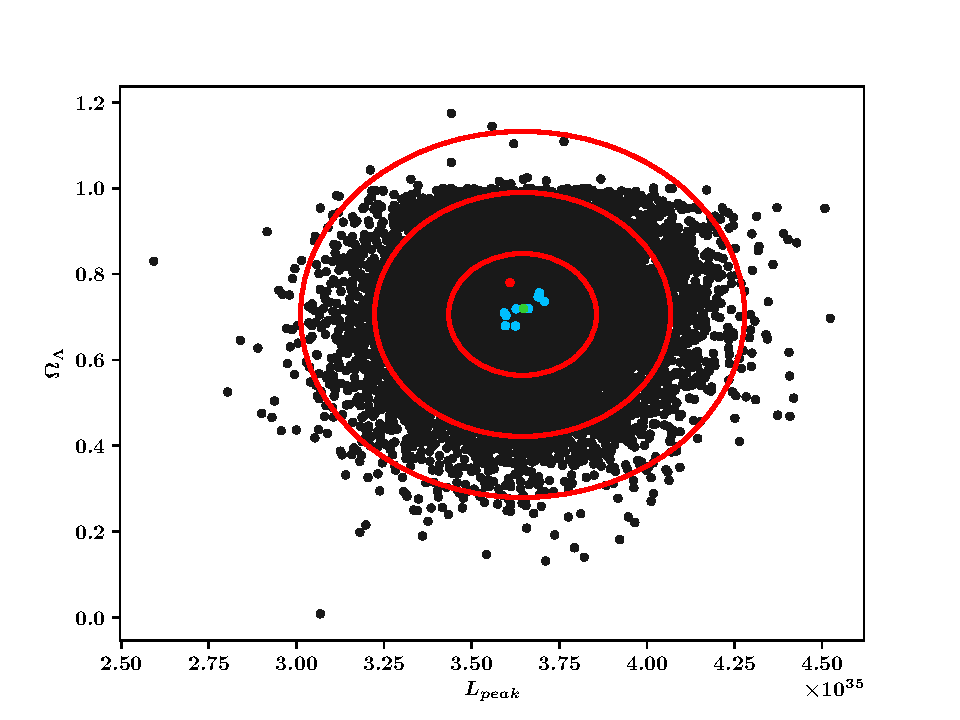
\includegraphics[width=9.25cm]{results/ol_lp_complete}
\caption[]{Plot showing the general forms of Type Ia supernovae in the B and V bands. Archival data was translated along the time and magnitude axes to produce the general forms of the light curves. The B band has been offset by a magnitude of $3$ to allow us to see both graphs clearly. The supernovae which were used to plot this graph are: \em{1994ae, 1994S, 1995bd, 1996bo, }\em  and \em{1998aq }\em \cite{jha, matheson}. }
\vspace{-3ex}
\label{fig:ol_lp_complete}
\end{center}
\end{figure}

sdfsadfasdf

\vspace{-3ex}
\subsection{$\chi^2$ Statistics} 
\vspace{-2ex}

asdasd

\vspace{-3ex}
\subsection{Bayesian Statistics} 
\vspace{-2ex}

asdasd


\begin{figure}[!h]
\begin{center}
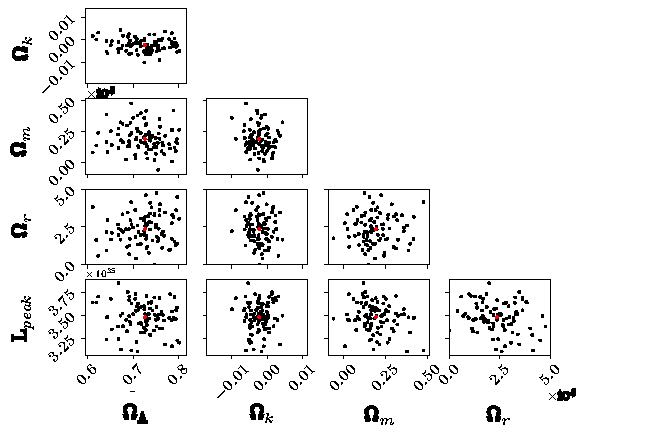
\includegraphics[width=9.25cm]{results/triangle}
\caption[]{Plot showing the general forms of Type Ia supernovae in the B and V bands. Archival data was translated along the time and magnitude axes to produce the general forms of the light curves. The B band has been offset by a magnitude of $3$ to allow us to see both graphs clearly. The supernovae which were used to plot this graph are: \em{1994ae, 1994S, 1995bd, 1996bo, }\em  and \em{1998aq }\em \cite{jha, matheson}. }
\vspace{-3ex}
\label{fig:triangle}
\end{center}
\end{figure}


sdfasdfsdfsad

\vspace{-3ex}
\subsection{Further Investigation} 
\vspace{-2ex}

asdasd

\vspace{-5ex}
\section{Conclusions}
\vspace{-2ex}

In conclusion, we have found that it is possible to constrain cosmological parameters of the universe using Type Ia supernova data.

\vspace{-3ex}
\bibliographystyle{abbrv}
\bibliography{supernova_cosmology}

\clearpage
\appendix

\vfill
\twocolumngrid
\vspace{-3ex}
\section{??}
\vspace{-2ex}



\clearpage
\end{document}